%%%%%%%%%%%%%%%%%%%%%%%%%%%%%%%%%%%%%%%%%%%%%%%%%%%%%%%%%%%%%%%%%%%%%%%%%%%%%%%%%%%%%%%%%%%%%%%%%%%%%%%%%%%%%%%%%%%%%%%%
\newpage
\chapter {\Large{Configuration}}

\begin{figure}[htbp]
	\centering
		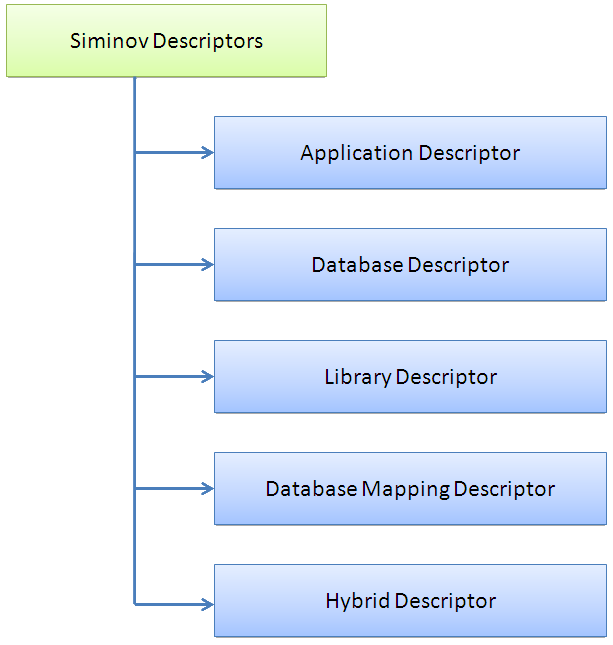
\includegraphics[height=8cm]{Resources/siminov_descriptors.png}
\end{figure}

\par
Siminov Framework works based on a set of defined descriptors which can be broadly classified as \textbf{ApplicationDescriptor.si.xml}, \textbf{DatabaseDescriptor.si.xml}, \textbf{LibraryDescriptor.si.xml}, \textbf{DatabaseMappingDescriptor.si.xml}, \textbf{HybridDescriptor.si.xml}

\par
All these descriptor should will be placed in application assests folder. 

\newpage
\begin{figure}[!htbp]
	\centering
		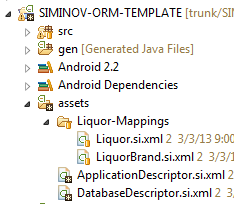
\includegraphics[height=8cm]{Resources/application_assests_structure.png}
\end{figure}


\begin{center}
	\colorbox{grey}{
		\parbox[t]{.8\linewidth}{
			\fontsize{11pt}{11pt}\selectfont % The first argument for fontsize is the font size of the text and the second is the line spacing - you may need to play with these for your particular title
			\vspace*{0.1cm} % Space between the start of the title and the top of the grey box
		
			\hfill \textbf{Note} \\

			\hfill 	
			\begin{enumerate}
			
				\item \small All descriptor file name should end with \textbf{.si.xml}.

			\end{enumerate}

			\vspace*{0.0cm} % Space between the end of the title and the bottom of the grey box
		}
	}

\end{center}



\newpage
\section{Application Descriptor (ApplicationDescriptor.si.xml) Configuration} 
	Application Descriptor is the one who connects application to Siminov framework. It provide basic information about application, which defines the behaviour of application.

\lstinputlisting[language=XML]{Resources/application_descriptor.txt}

\newpage
\textbf{Example}: ApplicationDescriptor.si.xml File Of Siminov Template Application.
\lstinputlisting[language=XML]{Resources/siminov_hybrid_template_application_descriptor.txt}

			\begin{center}
				\colorbox{grey}{
					\parbox[t]{.8\linewidth}{
						\fontsize{11pt}{11pt}\selectfont % The first argument for fontsize is the font size of the text and the second is the line spacing - you may need to play with these for your particular title
						\vspace*{0.1cm} % Space between the start of the title and the top of the grey box
		
						\hfill \textbf{Note} \\

			
						Application Developer can provide their own properties also, and by using following API's they can use properties.

						\hfill 	
						\begin{enumerate}
							\item \small Get Properties - getProperties(): It will return all properties associated with Application Descriptor.
							\item \small Get Property - getProperty(Name of Property): It will return property value associated with property name provided.
							\item \small Contains Property - containsProperty(Name of Property): It will return TRUE/FALSE whether property exists or not.
							\item \small Add Property - addProperty(Name of Property, Value of Property ): It will add new property to the  collection of Application Descriptor properties.
							\item \small Remove Property - removeProperty(Name of Property): It will remove property from Application Descriptor properties based on name provided.
						\end{enumerate}

						\vspace*{0.0cm} % Space between the end of the title and the bottom of the grey box
				}
			}

		\end{center}


\textbf{Application Descriptor Elements}: 

\begin{enumerate}
	
	\item \small General Properties About Application.
	
		\begin{enumerate}

			\item \small \textbf{name*} : Name of application. It is mandatory field. If any resources is created by Siminov then it will be under this folder name.

			\begin{figure}[htbp]
				\centering
					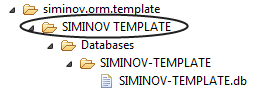
\includegraphics[height=3cm]{Resources/siminov_template_application_data_folder_structure_for_application_name.png}
			\end{figure}


			\item \small \textbf{description}: Description of application. It is optional field.
			\item \small \textbf{version}: Version of application. It is mandatory field. Default is 0.0.

		\end{enumerate}

	\item \small Framework Performance Properties.
		
		\begin{enumerate}

			\item \small \textbf{load\_initially}: \textit{TRUE}/\textit{FALSE}: ORM(Object Relational Mapping) to be done at start of application or at the time when its needed. It is optional field. By default its false, means mapping is done when its required. 

			\begin{center}
				\colorbox{grey}{
					\parbox[t]{.8\linewidth}{
						\fontsize{11pt}{11pt}\selectfont % The first argument for fontsize is the font size of the text and the second is the line spacing - you may need to play with these for your particular title
						\vspace*{0.1cm} % Space between the start of the title and the top of the grey box
		
						\hfill \textbf{Note} \\

						\hfill 	
						\begin{enumerate}
			
							\item \small If load\_initially is false then application will start quickly.

						\end{enumerate}

						\vspace*{0.0cm} % Space between the end of the title and the bottom of the grey box
				}
			}

		\end{center}

		
		\end{enumerate}

	\item \small Path Of Database Descriptor's Used In Application.

		\begin{itemize}

			\item \small Path of all database descriptor's used in application.
			\item \small Every database descriptor will have its own database object.
		
		\end{itemize}

	\item \small Event Handlers Implemented By Application 

		\begin{itemize}

			\item \small Siminov Framework provides two type of event handlers
			
				\begin{itemize}
					\item \small \textbf{ISiminovEvents}: It contains events associated with life cycle of Siminov Framework. such as \textbf{siminovInitialized}, \textbf{firstTimeSiminovInitialized}, \textbf{siminovStopped}.
					\item \small \textbf{IDatabaseEvents}: It contains events associated with database operations. such as \textbf{databaseCreated}, \textbf{databaseDropped}, \textbf{tableCreated}, \textbf{tableDropped}, \textbf{indexCreated}, 													\textbf{indexDropped}.
		
				\end{itemize}

			\item \small Application can implement these event handlers based on there requirement.

		\end{itemize}

		\begin{center}
			\colorbox{grey}{
				\parbox[t]{.8\linewidth}{
					\fontsize{11pt}{11pt}\selectfont % The first argument for fontsize is the font size of the text and the second is the line spacing - you may need to play with these for your particular title
					\vspace*{0.1cm} % Space between the start of the title and the top of the grey box
		
					\hfill \textbf{Note} \\

					\hfill 	
					\begin{enumerate}
			
						\item \small Event Handler can be define in both Native and Web.

						\item \small Native Event Handler: If you want to handle Event in Web then define Event Handler using JavaScript. Specify full Java class path name in ApplicationDescriptor.si.xml.

						\item \small Web Event Handler: If you want to handle Event in Web then define Event Handler using JavaScript. Specify only JavaScript Function name in ApplicationDescriptor.si.xml.

						\item \small Both (Native/Web) Event Handler: If you want to handle Event in both Native and Web then define Event Handler in both Java and JavaScript. Specify full Java class path and name in ApplicationDescriptor.si.xml, no need to define for JavaScript because Siminov will automatically accume same name for it.

					\end{enumerate}

					\vspace*{0.0cm} % Space between the end of the title and the bottom of the grey box
		}
}

\end{center}


\end{enumerate}

\begin{center}
	\colorbox{grey}{
		\parbox[t]{.8\linewidth}{
			\fontsize{11pt}{11pt}\selectfont % The first argument for fontsize is the font size of the text and the second is the line spacing - you may need to play with these for your particular title
			\vspace*{0.1cm} % Space between the start of the title and the top of the grey box
		
			\hfill \textbf{Note} \\

			\hfill 	
			\begin{enumerate}
			
				\item \small Application descriptor file name should always be same as ApplicationDescriptor.si.xml only.

				\item \small It should always be in root folder of application assests.

			\end{enumerate}

			\vspace*{0.0cm} % Space between the end of the title and the bottom of the grey box
		}
}

\end{center}

	\par
		\textbf{Example:} Siminov Template Application.
		\begin{figure}[htbp]
			\centering
				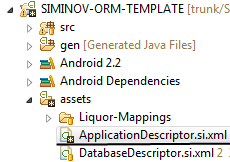
\includegraphics[height=4.5cm]{Resources/siminov_application_template_application_descriptor_path_example.png}
		\end{figure}


\newpage
\section{Database Descriptor (DatabaseDescriptor.si.xml) Configuration}
	Database Descriptor is the one who defines the schema of database.
	
\lstinputlisting[language=XML]{Resources/database_descriptor.txt}

\newpage
\textbf{Example}: DatabaseDescriptor.si.xml File Of Siminov Template Application.
\lstinputlisting[language=XML]{Resources/siminov_hybrid_template_database_descriptor.txt}


			\begin{center}
				\colorbox{grey}{
					\parbox[t]{.8\linewidth}{
						\fontsize{11pt}{11pt}\selectfont % The first argument for fontsize is the font size of the text and the second is the line spacing - you may need to play with these for your particular title
						\vspace*{0.1cm} % Space between the start of the title and the top of the grey box
		
						\hfill \textbf{Note} \\

			
						Application Developer can provide their own properties also, and by using following API's they can use properties.

						\hfill 	
						\begin{enumerate}
							\item \small Get Properties - getProperties(): It will return all properties associated with Database Descriptor.
							\item \small Get Property - getProperty(Name of Property): It will return property value associated with property name provided.
							\item \small Contains Property - containsProperty(Name of Property): It will return TRUE/FALSE whether property exists or not.
							\item \small Add Property - addProperty(Name of Property, Value of Property ): It will add new property to the  collection of Database Descriptor properties.
							\item \small Remove Property - removeProperty(Name of Property): It will remove property from Database Descriptor properties based on name provided.
						\end{enumerate}

						\vspace*{0.0cm} % Space between the end of the title and the bottom of the grey box
				}
			}

		\end{center}


\textbf{Database Descriptor Elements}: 

\begin{enumerate}

	\item \small General Properties About Database.

		\begin{enumerate}

			\item \small \textbf{database\_name*}: Name of database. It is mandatory field. All database files (.db)'s will be placed under the this folder name.

			\begin{figure}[htbp]
				\centering
					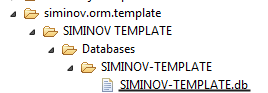
\includegraphics[height=3cm]{Resources/siminov_template_application_data_folder_structure_for_database_name.png}
			\end{figure}

			\item \small \textbf{type}: It defines the type of database. It is optional field. Default is sqlite.

			\item \small \textbf{description}: Description of database. It is optional field.
			\item \small \textbf{is\_locking\_required}: \textbf{TRUE}/\textbf{FALSE}, Control whether or not the database is made thread-safe by using locks around critical sections. 
				
				\par
				This is pretty expensive, so if you know that your DB will only be used by a multi threads then you should set this to true. 

				\par
				The default is false. It is optional field. 
			
			\begin{center}
				\colorbox{grey}{
					\parbox[t]{.8\linewidth}{
						\fontsize{11pt}{11pt}\selectfont % The first argument for fontsize is the font size of the text and the second is the line spacing - you may need to play with these for your particular title
						\vspace*{0.1cm} % Space between the start of the title and the top of the grey box
		
						\hfill \textbf{Note} \\

						\hfill 	Siminov does not provide any security for database. If you want your database data needs to encrypted, then you can include SQLCipher implementation provided by Siminov framework in your application. For more detail see SQLCipher Encryption section of this developer guide.

						\vspace*{0.0cm} % Space between the end of the title and the bottom of the grey box
					}
			}

			\end{center}

			\item \small \textbf{external\_storage}:It specifies whether database resources needs to be saved on external storage or not (SDCard). It is optinal field. Default is false.

		\end{enumerate}


	\item \small Paths Of Database Mapping Descriptor Needed Under This Database Descriptor. 

			\begin{center}
				\colorbox{grey}{
					\parbox[t]{.8\linewidth}{
						\fontsize{11pt}{11pt}\selectfont % The first argument for fontsize is the font size of the text and the second is the line spacing - you may need to play with these for your particular title
						\vspace*{0.1cm} % Space between the start of the title and the top of the grey box
		
						\hfill \textbf{Note} \\

						\hfill 

						\begin{enumerate}

							\item \small Provide full database mapping descriptor file path if you have used xml format to define ORM.

							\item \small Provide full class path of database mapping descriptor POJO class if you have used annotation to define ORM.
	
						\end{enumerate}

						\vspace*{0.0cm} % Space between the end of the title and the bottom of the grey box
					}
			}

			\end{center}

	\item \small Paths Of Library Descriptor Needed Under This Database Descriptor.

			\begin{center}
				\colorbox{grey}{
					\parbox[t]{.8\linewidth}{
						\fontsize{11pt}{11pt}\selectfont % The first argument for fontsize is the font size of the text and the second is the line spacing - you may need to play with these for your particular title
						\vspace*{0.1cm} % Space between the start of the title and the top of the grey box
		
						\hfill \textbf{Note} \\

						\hfill 

						\begin{enumerate}

							\item \small Provide full package name under which LibraryDescriptor.si.xml file is placed.

							\item \small Siminov framework will automatically read LibraryDescriptor.si.xml file defined under package name provided.
	
						\end{enumerate}

						\vspace*{0.0cm} % Space between the end of the title and the bottom of the grey box
					}
			}

			\end{center}

\end{enumerate}


	\begin{center}
		\colorbox{grey}{
			\parbox[t]{.8\linewidth}{
				\fontsize{11pt}{11pt}\selectfont % The first argument for fontsize is the font size of the text and the second is the line spacing - you may need to play with these for your particular title
				\vspace*{0.1cm} % Space between the start of the title and the top of the grey box
		
				\hfill \textbf{Note} \\

				\hfill 

				\begin{enumerate}

					\item \small You can specify any name for DatabaseDescriptor.si.xml file.

					\item \small If any database folder is created, it will be on the name of database defined in DatabaseDescriptor.si.xml file.
	
				\end{enumerate}

				\vspace*{0.0cm} % Space between the end of the title and the bottom of the grey box
			}
	}

\end{center}

\newpage
	\par
		\textbf{Example:} DatabaseDescriptor.si.xml file path
		\begin{figure}[htbp]
			\centering
				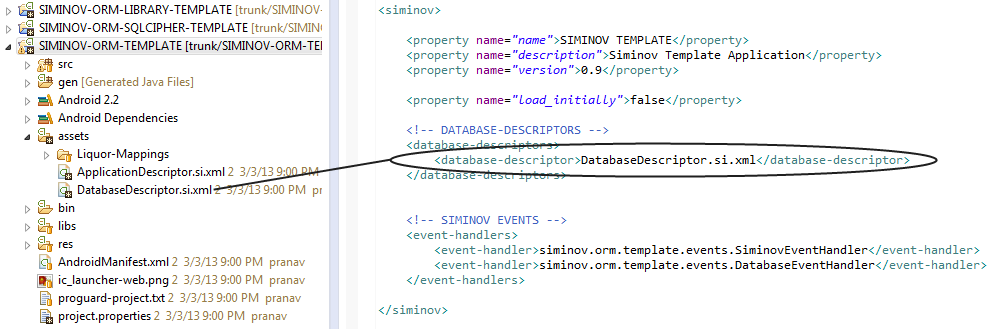
\includegraphics[height=6cm]{Resources/siminov_template_application_database_descriptor_path_example.png}
		\end{figure}




\newpage
\section{Library Descriptor (LibraryDescriptor.si.xml) Configuration}
	Library Descriptor is the one who defines the properties of library.

\lstinputlisting[language=XML]{Resources/library_descriptor.txt}

\textbf{Example}: LibraryDescriptor.si.xml File Of Siminov Library Template.
\lstinputlisting[language=XML]{Resources/siminov_library_template_library_descriptor.txt}

			\begin{center}
				\colorbox{grey}{
					\parbox[t]{.8\linewidth}{
						\fontsize{11pt}{11pt}\selectfont % The first argument for fontsize is the font size of the text and the second is the line spacing - you may need to play with these for your particular title
						\vspace*{0.1cm} % Space between the start of the title and the top of the grey box
		
						\hfill \textbf{Note} \\

			
						Application Developer can provide their own properties also, and by using following API's they can use properties.

						\hfill 	
						\begin{enumerate}
							\item \small Get Properties - getProperties(): It will return all properties associated with Library Descriptor.
							\item \small Get Property - getProperty(Name of Property): It will return property value associated with property name provided.
							\item \small Contains Property - containsProperty(Name of Property): It will return TRUE/FALSE whether property exists or not.
							\item \small Add Property - addProperty(Name of Property, Value of Property ): It will add new property to the  collection of Library Descriptor properties.
							\item \small Remove Property - removeProperty(Name of Property): It will remove property from Library Descriptor properties based on name provided.
						\end{enumerate}

						\vspace*{0.0cm} % Space between the end of the title and the bottom of the grey box
				}
			}

		\end{center}


\newpage
\textbf{Library Descriptor Elements}: 

\begin{enumerate}

	\item \small General Properties Of Library.
		
		\begin{enumerate}

			\item \small \textbf{name*}: Name of library. It is mandatory field.
			\item \small \textbf{description}: Description of library. It is optional field.
		
		\end{enumerate}

	\item \small Database Mapping Paths Needed Under This Database Descriptor.	

			\begin{center}
				\colorbox{grey}{
					\parbox[t]{.8\linewidth}{
						\fontsize{11pt}{11pt}\selectfont % The first argument for fontsize is the font size of the text and the second is the line spacing - you may need to play with these for your particular title
						\vspace*{0.1cm} % Space between the start of the title and the top of the grey box
		
						\hfill \textbf{Note} \\

						\hfill 

						\begin{enumerate}

							\item \small Provide full database mapping descriptor file path if you have used xml format to define ORM.

							\item \small Provide full class path of database mapping descriptor POJO class if you have used annotation to define ORM.
	
						\end{enumerate}

						\vspace*{0.0cm} % Space between the end of the title and the bottom of the grey box
					}
			}

			\end{center}

\end{enumerate}

	\begin{center}
		\colorbox{grey}{
			\parbox[t]{.8\linewidth}{
				\fontsize{11pt}{11pt}\selectfont % The first argument for fontsize is the font size of the text and the second is the line spacing - you may need to play with these for your particular title
				\vspace*{0.1cm} % Space between the start of the title and the top of the grey box
		
				\hfill \textbf{Note} \\

				\hfill 

				\begin{enumerate}

					\item \small Library descriptor file name should be same as LibraryDescriptor.si.xml.

					\item \small It should always be in root package specified in DatabaseDescriptor.si.xml file.
	
				\end{enumerate}

				\vspace*{0.0cm} % Space between the end of the title and the bottom of the grey box
			}
		}

\end{center}



		\par
		\textbf{Example:} LibraryDescriptor.si.xml file path
		\begin{figure}[htbp]
			\centering
				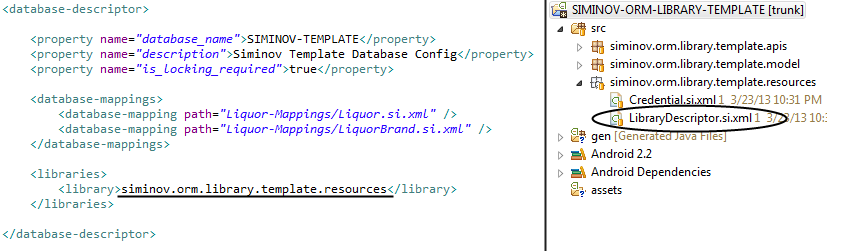
\includegraphics[height=6.2cm]{Resources/siminov_library_template_path_example.png}
		\end{figure}



\newpage
\section{Database Mapping Descriptor (DatabaseMappingDescriptor.si.xml) Configuration}
	
Database Mapping Descriptor is one which does ORM, it maps Java/JavaScript POJO class to database table.
\lstinputlisting[language=XML]{Resources/database_mapping_descriptor.txt}


\textbf{Example}: DatabaseMappingDescriptor.si.xml File Of Siminov Hybrid Template.
\lstinputlisting[language=XML]{Resources/siminov_hybrid_template_application_liquor_database_mapping_descriptor.txt}


\newpage
\textbf{Database Mapping Descriptor Elements}:



\begin{enumerate}

	\item \small \textbf{TABLE TAG}: It map database table to its corresponding POJO class.

		\begin{enumerate}

			\item \small \textbf{table\_name*}: Name of table. It is mandatory field.
			\item \small \textbf{class\_name*}: Name of Java/JavaScript POJO class name which is to be mapped to table name. It is mandatory field.

	\begin{center}
		\colorbox{grey}{
			\parbox[t]{.8\linewidth}{
				\fontsize{11pt}{11pt}\selectfont % The first argument for fontsize is the font size of the text and the second is the line spacing - you may need to play with these for your particular title
				\vspace*{0.1cm} % Space between the start of the title and the top of the grey box
		
				\hfill \textbf{Note} \\

				\hfill 

				\begin{enumerate}

					\item \small POJO Class can be define in both Native and Web.
					
					\item \small Native Class: If you mapped POJO class is in Native then use Java to define class. Specify full Java class path and name in class\_name TAG.

					\item \small Web Class: If you have mapped POJO class is in Web then use JavaScript to define class. Specify only JavaScript Function name in class\_name TAG.

					\item \small Both (Native/Web) Class: If you mapped POJO class is in both Native and Web then both Java and JavaScript to define classes. Specify full Java class path and name in class\_name TAG, no need to define for JavaScript because Siminov will automatically assume same name for it.

	
				\end{enumerate}

				\vspace*{0.0cm} % Space between the end of the title and the bottom of the grey box
			}
		}

	\end{center}
			
		\end{enumerate}


	\item \small \textbf{COLUMN TAG}: It map database table column to its corresponding variable of POJO class.

		\begin{enumerate}

			\item \small \textbf{column\_name*}: Name of column. It is mandatory field.
			\item \small \textbf{variable\_name*}: Name of variable. It is mandatory field.

		\end{enumerate}

		
		\par
		\textbf{Properties Of Column Tag}
	
		\begin{enumerate}

			\item \small \textbf{type*}: Variable data type. It is mandatory property. 


	\begin{center}
		\colorbox{grey}{
			\parbox[t]{.8\linewidth}{
				\fontsize{11pt}{11pt}\selectfont % The first argument for fontsize is the font size of the text and the second is the line spacing - you may need to play with these for your particular title
				\vspace*{0.1cm} % Space between the start of the title and the top of the grey box
		
				\hfill \textbf{Note} \\

				\hfill 

				\begin{enumerate}
		
					\item \small POJO Class can be define in both Native and Web.

					\item \small Native Class: If you have mapped POJO class in Native then specify Java Variable data type.

					\begin{enumerate}

						\item \small 

					\end{enumerate} 
						
				\end{enumerate}

				\vspace*{0.0cm} % Space between the end of the title and the bottom of the grey box
			}
		}

	\end{center}

				

				\par
				For more details see Data Type section of this developer guide.
			
			\item \small \textbf{primary\_key}: \textit{TRUE}/\textit{FALSE}. It defines wheather the column is primary key of table or not. It is optional property. Default value is false.
			\item \small \textbf{not\_null}: \textit{TRUE}/\textit{FALSE}. It defines wheather the column value can be empty or not. It is optional property. Default value is false.
			\item \small \textbf{unique}: \textit{TRUE}/\textit{FALSE}. It defines wheather the column value should be unique or not. It is optional property. Default value is false.
			\item \small \textbf{default}: It define the default value of column. It is optional property.
			\item \small \textbf{check}: It is used to put condition on column value. It is optional property.

		\end{enumerate}

			\begin{center}
				\colorbox{grey}{
					\parbox[t]{.8\linewidth}{
						\fontsize{11pt}{11pt}\selectfont % The first argument for fontsize is the font size of the text and the second is the line spacing - you may need to play with these for your particular title
						\vspace*{0.1cm} % Space between the start of the title and the top of the grey box
		
						\hfill \textbf{Note} \\

			
						Application Developer can provide their own properties also, and by using following API's they can use properties.

						\hfill 	
						\begin{enumerate}
							\item \small Get Properties - getProperties(): It will return all properties associated with Database Mapping Descriptor Column.
							\item \small Get Property - getProperty(Name of Property): It will return property value associated with property name provided.
							\item \small Contains Property - containsProperty(Name of Property): It will return TRUE/FALSE whether property exists or not.
							\item \small Add Property - addProperty(Name of Property, Value of Property ): It will add new property to the  collection of Database Mapping Descriptor Column properties.
							\item \small Remove Property - removeProperty(Name of Property): It will remove property from Database Mapping Descriptor Column properties based on name provided.
						\end{enumerate}

						\vspace*{0.0cm} % Space between the end of the title and the bottom of the grey box
				}
			}

		\end{center}


	\item \small \textbf{INDEX TAG}: It defines the stucture of  index needed on the table.

		\begin{enumerate}

			\item \small \textbf{name*}: Name of the index. It is mandatory field.
			\item \small \textbf{unique}: \textit{TRUE}/\textit{FALSE}. It defines wheather index needs to be unique or not. It is not mandatory property. Default value is false.
				
				\par
				(A unique index guarantees that the index key contains no duplicate values and therefore every row in the table is in some way unique). 

		\end{enumerate}


		\par
		\textbf{Index Column Tag}

		\begin{enumerate}

			\item \small \textbf{column}: Name of columns included in index. Atleast one column should be included.

		\end{enumerate}
		

	
	\item \small \textbf{RELATIONSHIPS TAG}: It defines relationship between object.

		\par
		Relationship can be of four types:

		\begin{enumerate}

			\item \small \textbf{ONE-TO-ONE}: \textit{\[<one-to-one>\]} In a one-to-one relationship, each row in one database table is linked to 1 and only 1 other row in another table.

			\item \small \textbf{ONE-TO-MANY}: \textit{\[<one-to-many>\]} In a one-to-many relationship, each row in the related to table can be related to many rows in the relating table. This effectively save storage as the related record does not need to be stored multiple times in the relating table.

			\item \small \textbf{MANY-TO-ONE}: \textit{\[<many-to-one>\]} In a many-to-one relationship one entity (typically a column or set of columns) contains values that refer to another entity (a column or set of columns) that has unique values.
	
			\item \small \textbf{MANY-TO-MANY}: \textit{\[<many-to-many>\]} In a many-to-many relationship, one or more rows in a table can be related to 0, 1 or many rows in another table. A mapping table is required in order to implement such a relationship.
	
		\end{enumerate}

			
		\textbf{Relationship Attributes}

		\begin{enumerate}

			\item \small \textbf{refer*}: Name of variable which needs to be mapped. It is mandatory field.

			\item \small \textbf{refer\_to*}: Class name of mapped variable. It is mandatory field.

			\item \small \textbf{on\_update}: \textit{cascade}/\textit{restrict}/\textit{no\_action}/\textit{set\_null}/\textit{set\_default}. It defines action needs to be done, when update occur.

			\item \small \textbf{on\_delete}: \textit{cascade}/\textit{restrict}/\textit{no\_action}/\textit{set\_null}/\textit{set\_default}. It defines action needs to be done, when delete occur.
		
		\end{enumerate}

		\textbf{Relationship Properties}

		\begin{enumerate}

			\item \small \textbf{load}: It defines whether it need to be load or not.
			
		\end{enumerate}
		
\end{enumerate}

\newpage
\begin{center}
		\colorbox{grey}{
			\parbox[t]{.8\linewidth}{
				\fontsize{11pt}{11pt}\selectfont % The first argument for fontsize is the font size of the text and the second is the line spacing - you may need to play with these for your particular title
				\vspace*{0.1cm} % Space between the start of the title and the top of the grey box
		
				\hfill \textbf{Note} \\

				\hfill 

				\begin{enumerate}

					\item \small Application developer can assign any name to DatabaseMappingDescriptor.si.xml file.

					\item \small It descriptor file should be in same place as per defined in DatabaseDescriptor.si.xml file.
	
				\end{enumerate}

				\vspace*{0.0cm} % Space between the end of the title and the bottom of the grey box
			}
		}

\end{center}

		\par
		\textbf{Example:} DatabaseMappingDescriptor.si.xml file path
		\begin{figure}[htbp]
			\centering
				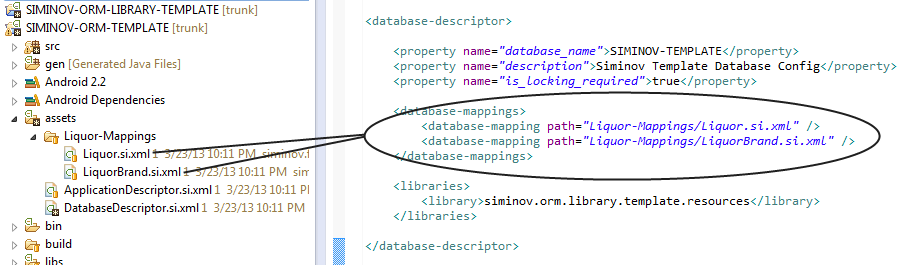
\includegraphics[height=6cm]{Resources/siminov_template_database_descriptor_mapping_path_example.png}
		\end{figure}


\newpage
\section{Database Mapping Descriptor Through Annotation}
Annotation is another way to do ORM, it maps POJO class to database table.

\par
(Annotations provide data about a program that is not part of the program itself. They have no direct effect on the operation of the code they annotate)

\lstinputlisting[language=Java]{Resources/database_mapping_descriptor_annotation.txt}

\textbf{Example}: Liquor Class Of Siminov Template Application.
\lstinputlisting[language=XML]{Resources/siminov_template_application_liquor_annotation_class.txt}

\newpage
\textbf{Different Annotation Tags}:

\begin{enumerate}

	\item \small \textbf{@Table}: It map database table to its corresponding POJO class.
		
		\begin{enumerate}

			\item \small \textbf{tableName*}: Name of table. It is mandatory field.

		\end{enumerate}
	

	\item \small \textbf{@Indexes}: It contain all index required on table.


	\item \small \textbf{@Index}: It defines the stucture of  index needed on the table.

		\begin{enumerate}

			\item \small \textbf{name*}: Name of the index. It is mandatory field.
			\item \small \textbf{unique}: \textit{TRUE}/\textit{FALSE}. It defines wheather index needs to be unique or not. It is not mandatory property. Default value is false.
				
				\par
				(A unique index guarantees that the index key contains no duplicate values and therefore every row in the table is in some way unique). 


		\end{enumerate}

		
		\par
		\textbf{Index Column Tag}

		\begin{enumerate}

			\item \small \textbf{column}: Name of columns included in index. Atleast one column should be included.

		\end{enumerate}

	\item \small \textbf{@Column}: It map database table column to its corresponding variable of POJO class.

		\begin{enumerate}

			\item \small \textbf{columnName*}: Name of column. It is mandatory field.

		\end{enumerate}

		\par
		\textbf{Properties Of Column: @Properties}: It contain all properties needed by column.
	
		\par
		\textbf{Properties Of Column Tag: @Property}: This tag defines a perticular property of column.

		\begin{enumerate}

			\item \small \textbf{primary\_key} | \textbf{ColumnProperty}.\textbf{PRIMARY\_KEY}: \textit{TRUE}/\textit{FALSE}. It defines wheather the column is primary key of table or not. It is optional property. Default value is false.
			\item \small \textbf{not\_null} | \textbf{ColumnProperty}.\textbf{NOT\_NULL}: \textit{TRUE}/\textit{FALSE}. It defines wheather the column value can be empty or not. It is optional property. Default value is false.
			\item \small \textbf{unique} | \textbf{ColumnProperty}.\textbf{UNIQUE}: \textit{TRUE}/\textit{FALSE}. It defines wheather the column value should be unique or not. It is optional property. Default value is false.
			\item \small \textbf{default} | \textbf{ColumnProperty}.\textbf{DEFAULT}: It define the default value of column. It is optional property.
			\item \small \textbf{check} | \textbf{ColumnProperty}.\textbf{CHECK}: It is used to put condition on column value. It is optional property.

		\end{enumerate}

	\item \small \textbf{@OneToOne}: This tag defines one-to-one relationship, where each row in one database table is linked to 1 and only 1 other row in another table.

		\begin{enumerate}

			\item \small \textbf{onUpdate}: \textit{cascade}/\textit{restrict}/\textit{no\_action}/\textit{set\_null}/\textit{set\_default}. It defines action needs to performed, when update occur. 
			\item \small \textbf{onDelete}: \textit{cascade}/\textit{restrict}/\textit{no\_action}/\textit{set\_null}/\textit{set\_default}. It defines action needs to be performed, when delete occur.		

		\end{enumerate}


	\item \small \textbf{@OneToMany}: This tag defines one-to-many relationship, where each row in the related to table can be related to many rows in the relating table. This effectively save storage as the related record does not need to be stored multiple times in the relating table.
	
		\begin{enumerate}

			\item \small \textbf{onUpdate}: \textit{cascade}/\textit{restrict}/\textit{no\_action}/\textit{set\_null}/\textit{set\_default}. It defines action needs to performed, when update occur. 
			\item \small \textbf{onDelete}: \textit{cascade}/\textit{restrict}/\textit{no\_action}/\textit{set\_null}/\textit{set\_default}. It defines action needs to be performed, when delete occur.		

		\end{enumerate}

	\item \small \textbf{@ManyToOne}: This tag defines one-to-many relationship, where one entity (typically a column or set of columns) contains values that refer to another entity. (a column or set of columns) that has unique values.
	

		\begin{enumerate}

			\item \small \textbf{onUpdate}: \textit{cascade}/\textit{restrict}/\textit{no\_action}/\textit{set\_null}/\textit{set\_default}. It defines action needs to performed, when update occur. 
			\item \small \textbf{onDelete}: \textit{cascade}/\textit{restrict}/\textit{no\_action}/\textit{set\_null}/\textit{set\_default}. It defines action needs to be performed, when delete occur.		

		\end{enumerate}

	\item \small \textbf{@ManyToMany}: This tag defines one-to-many relationship, where one or more rows in a table can be related to 0, 1 or many rows in another table. A mapping table is required in order to implement such a relationship.

		\begin{enumerate}

			\item \small \textbf{onUpdate}: \textit{cascade}/\textit{restrict}/\textit{no\_action}/\textit{set\_null}/\textit{set\_default}. It defines action needs to performed, when update occur. 
			\item \small \textbf{onDelete}: \textit{cascade}/\textit{restrict}/\textit{no\_action}/\textit{set\_null}/\textit{set\_default}. It defines action needs to be performed, when delete occur.		

		\end{enumerate}

	\par
		\textbf{RELATIONSHIP PROPERTY TAG}: @RelationshipProperty

			\begin{enumerate}

				\item \small \textbf{load}: \textit{TRUE/FALSE}, It defines whether it need to be load or not.	

			\end{enumerate}


\end{enumerate}
